
 No quesito excesso de pó, uma das melhores correções está na aplicação de um revestimento primário selante. No caso dos solos siltosos este problema se agrava, pois a formação de poeira é mais intensa e a capacidade de suporte deste material é baixa. Neste caso, além do revestimento primário, é necessário o reforço do subleito.
 
 Para a curva fechada a solução técnica deve ser baseada nas características oferecidas pelo local, pois muitas vezes a tomada de decisão baseada nesses requisitos não é suficiente quando se emprega os materiais locais disponíveis. Dessa forma, a implantação de tal medida corretiva fica a cargo da viabilidade do processo diante dos recursos presentes para a execução da obra.
 
 Porém, supondo que ela atenda os requisitos locais para a correção do problema seria conveniente o afastamento lateral dos obstáculos em curva para aumentar a linha de visão do condutor.
 
 \begin{figure}[ht]
 	\centering
 	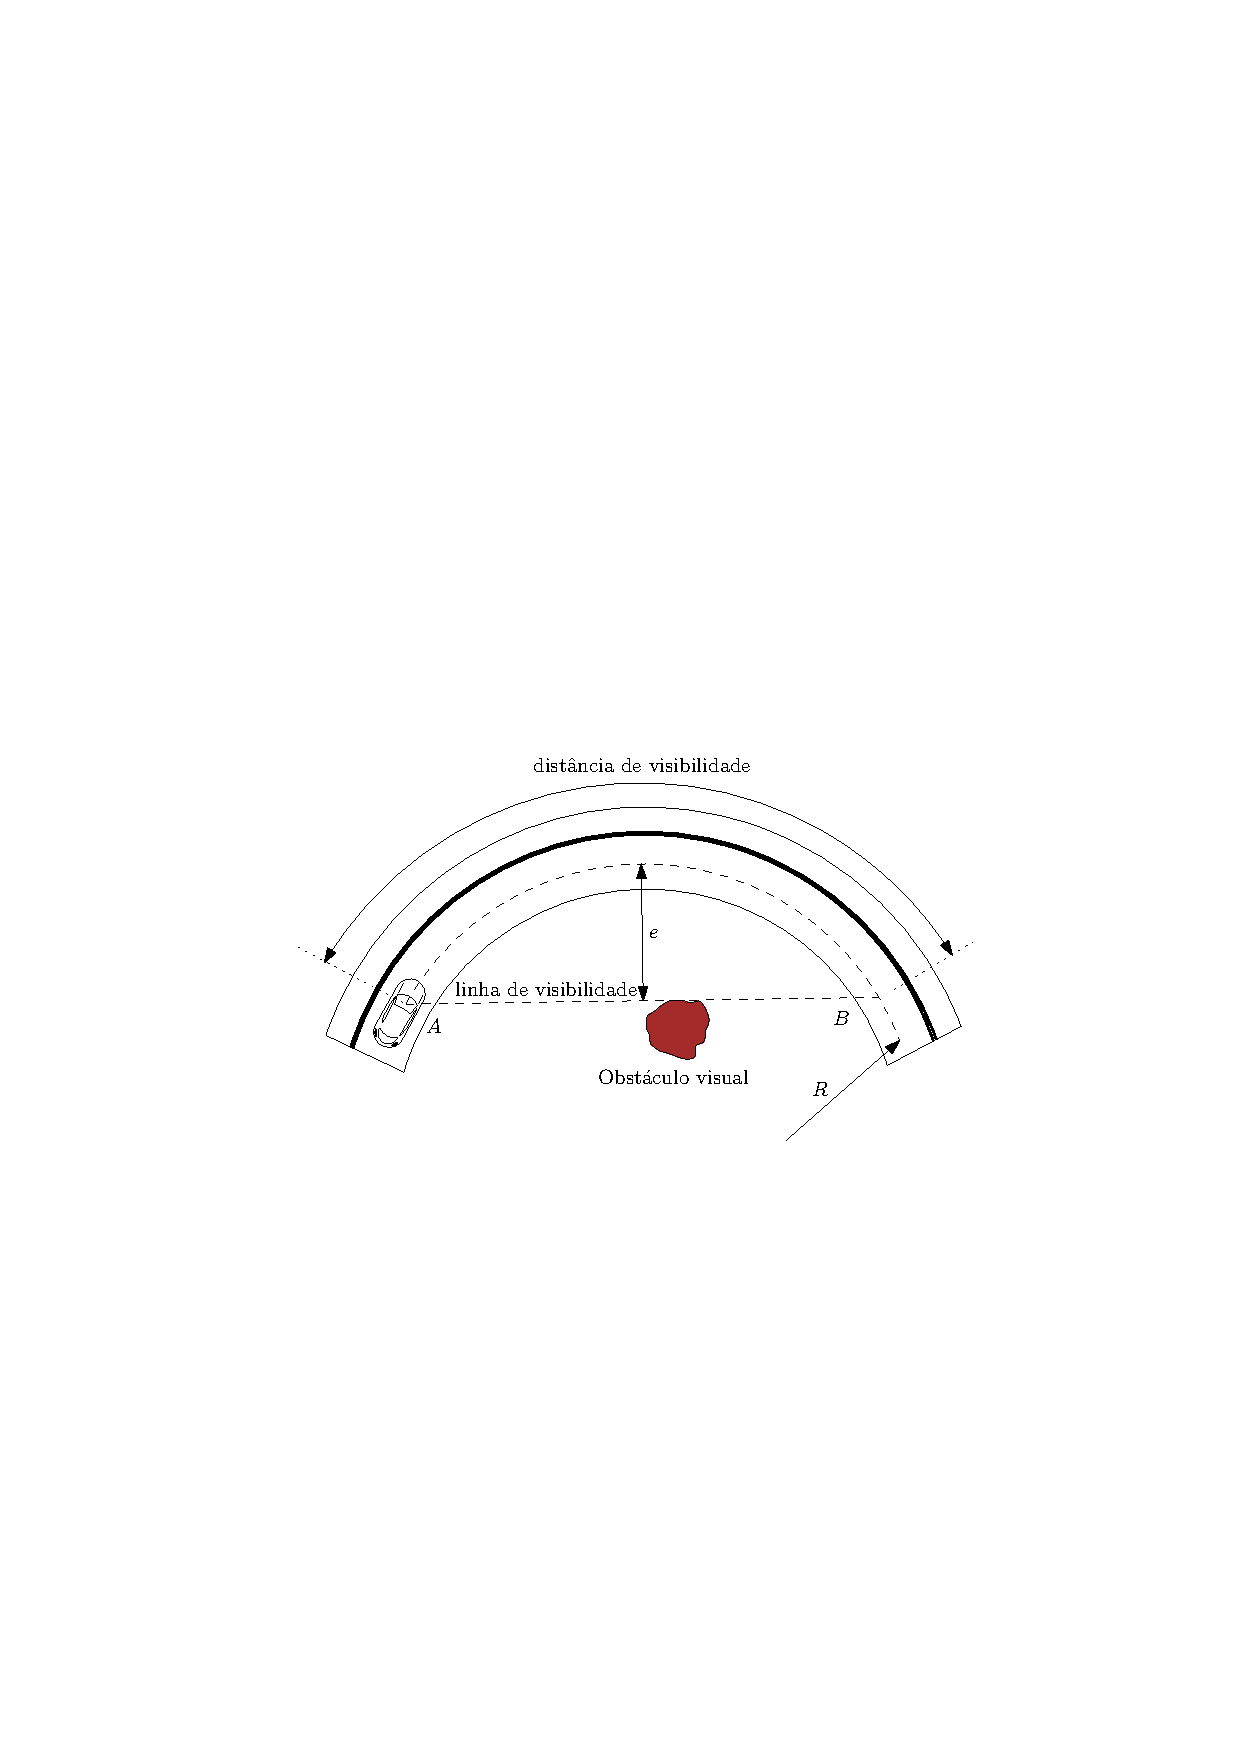
\includegraphics[scale=1.3]{../../images/draw_1}
 	\caption{Vista esquemática representando a influência que um obstáculo exerce na visibilidade do motorista.}
 \end{figure}